\documentclass{beamer}
\usetheme{Boadilla}
% \usepackage[a4paper, tmargin=1in, bmargin=1in]{geometry}
\usepackage[utf8]{inputenc}
\usepackage{graphicx}
\usepackage{parskip}
\usepackage{pdflscape}
\usepackage{listings}
\usepackage{hyperref}
\usepackage{float}
\usepackage{caption}
\usepackage{subcaption}
\usepackage{amssymb}
\usepackage{multirow}
% \mode<presentation>{
%     \AtBeginSection[]
%     {
%     \begin{frame}[allowframebreaks]{Outline}
%     \tableofcontents[currentsection]
%     \end{frame}
%     }
% }
% \AtBeginSubsection[
%   {\frame<beamer>{\frametitle{Outline}
%     \tableofcontents[currentsection,currentsubsection]}}%
% ]%
% {
%   \frame<beamer>{
%     \frametitle{Outline}
%     \tableofcontents[currentsection,currentsubsection]}
% }

\title{ECG Disease Classification Using Graph Convolution Networks}
% \subtitle{Using Beamer}
\author[Arka Sadhu]{Arka Sadhu \\ Supervised by Prof. Subhasis Chaudhuri}
\institute{IIT Bombay}
\date{\today}


\begin{document}
% document goes here


\begin{frame}
\titlepage
\end{frame}

% \begin{frame}
% \frametitle{Outline}
% \tableofcontents
% \end{frame}

\section{Problem Statement and Motivation}

% \subsection{Why GCN}
\begin{frame}
  \frametitle{Problem Statement}
  \begin{itemize}
  \item We are given annotated ECG data, i.e. ECG recordings along with the corresponding disease.
  \item Given a new ECG sample, we want to clasify into the different categories of disease.
  \item In current framework, only considered one-label classification, not multi-labeling.
  \item Previous work can be classified into two categories:
    \begin{itemize}
    \item Signal Processing techniques for good feature extraction (eg. QRS peak detection) coupled with standard Machine Learning approaches.
    \item Neural Networks for extraction of feature as well as for classification (eg. Convolutional Networks as there is periodicity associated)
    \end{itemize}
  \item We want to extend the success of Neural Networks to this task as well.
  \end{itemize}
\end{frame}

\begin{frame}
  \frametitle{Motivation}
  We wish to classify the disease of person based on raw ECG data.
  \begin{itemize}
  \item The main motivation comes from being able to capture real time ECG data and use that monitor the occurence of any heart related problem in the patient.
  \item This can also serve as a second opinion to the doctor.
  \end{itemize}
  Problems with Existing Methods:
  \begin{itemize}
  \item Signal Processing Techniques often may be computationally expensive and cannot work in real time.
  \item Need extremely high accuracy perhaps so as to not to trigger false alarms.
  \end{itemize}
\end{frame}

\begin{frame}
  \frametitle{Heart diseases considered}
  The following heart diseases are considered:
  \begin{itemize}
  \item Myocardial Infarction
  \item Cardiomyopathy \ Heart failure
  \item Bundle branch block
  \item Dysrhythmia
  \item Myocarditis
  \end{itemize}
  Currently, we are bothered only with Myocardial Infarction which is major part of the PTB dataset (described next).
\end{frame}

\begin{frame}
  \frametitle{Methodology}
  The following methodology is followed:
  \begin{itemize}
  \item First we analyze using simple Convolutional Neural Networks [CNN] for our problem. CNN are a good starting point as they are well known for their spatial invariance which in 1D can be considered as the temporal invariance which is something required in a continuous ECG data.
  \item Next we hope to understand what things CNN is able to learn well and what it is not. In particular we want to identify some Ad-Hocs which lead to better convergence of the Neural Network.
  \item Then we want to know the bottleneck of the learning and what we can do to improve it, which introduces us to Graph CNN.
  \end{itemize}
\end{frame}

\section{CNN on ECG}
\begin{frame}
  \frametitle{Dataset}
  The dataset used for experiments is the PTB database from Physionet repository.
  \begin{itemize}
  \item Consists of 15 channels (12 for conventional ecgs, 3 frank leads).
  \item Resolution is 16bit and sampling rate is 1kHz.
  \item Total 549 recordings from 290 subjects. 148 are diagnosed with Myocardial Infarction (MI).
  \item We use parts of each classification for training and rest for testing.
  \end{itemize}
\end{frame}

\begin{frame}
  \frametitle{CNN on ECG}
  A simple Convolutional Network is tested on ECG.
  \begin{itemize}
  \item Architecture adopted is 1D version of the LeNet architecture. The network is :
    $$conv -> max pool -> conv -> max pool -> fc -> fc -> softmax$$
  \item Base implementation results in accuracy around 80-87\%.
  \item Some Ad-Hocs are required to get better results.
  \end{itemize}
\end{frame}

\begin{frame}
  \frametitle{CNN on ECG (contd.)}
  \begin{itemize}
  \item Since data is not so much, each ECG data is pre-processed by taking the samples upto fixed period only (eg. 38000 points are broken into 27 partitions).
  \item On top of each convolution layer, we add a batch normalization. This gives accuracy boost upto 93\%-94\%
  \item State of the Art to the best of my knowledge on the PTB dataset is 96\% [1]
  \item It is also noted that using more number of channels doesn't lead to increase in the accuracy.
  \end{itemize}
  We would like to do better.
\end{frame}

\begin{frame}
  \frametitle{Results on using CNNs on ECG}
  \begin{figure}[H]
    \centering
    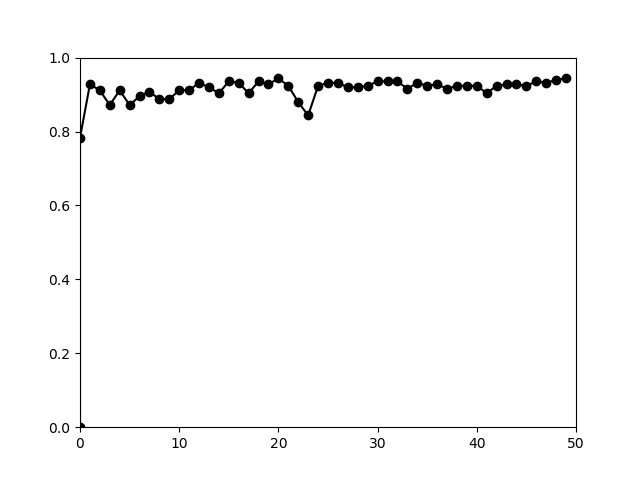
\includegraphics[scale=0.5]{images/bn_before_relu_acc_94_3}
    \caption{Accuracy of validation set vs Number of epochs}
    \label{fig:1}
  \end{figure}
\end{frame}

\section{Graph CNN}
\begin{frame}
  \frametitle{Exploiting Data from Different Channels}
  \begin{itemize}
  \item We note that the ECG leads are put at particular locations. We would like to be able to use the underlying spatial distribution as well and incorporate data from the different leads. This is something that the standard CNN can not do.
  \item For this reason we go to Graph Convolutional Networks. This can be viewed as a generalization of CNN to non-euclidean spaces.
  \item It is not trivial to generalize CNN to non-euclidean spaces.
  \end{itemize}
\end{frame}

\begin{frame}
  \frametitle{Graph CNN (Optional)}
  Two main approaches to Graph CNN
  \begin{itemize}
  \item Spectral Approach [ChebNet, NIPS2016][2]
    \begin{itemize}
    \item Basic Idea : Use graph laplacian and do convolution operation in the spectral domain.
    \end{itemize}
  \item Spatial Approach [MoNet, CVPR2017][3]
    \begin{itemize}
    \item Basic Idea : Use a local manifold and learn in polar coordinates.
    \end{itemize}
  \end{itemize}
  A limitation of Spectral Approach is that the underlying graph should be fixed, which is fortunately the case for ECG.
\end{frame}

\begin{frame}
  \frametitle{ChebNet (Optional)}
  Main Ideas in ChebNet:
  \begin{itemize}
  \item Uses graph laplacian and computes convolution in the fourier domain (using graph fourier transform).
  \item Restricts convolution to a local domain (k-hops) even when using the spectral approach.
  \item Efficient computation of the graph convoluion using the Chebyshev Polynomials.
  \item Efficient coarsening and pooling operation on graphs.
  \end{itemize}
  Main Limitation:
  \begin{itemize}
  \item The graph should be fixed. Cannot learn on multiple graphs.
  \end{itemize}
\end{frame}

\begin{frame}
  \frametitle{ChebNet on ECG data}
  This is still Work In Progress. Code is ready and small bug fixes are to be made.
  % \begin{itemize}
  % \item Main limitation is that the code is
  % \end{itemize}
\end{frame}


\begin{frame}
  \frametitle{Main Limitations of the Approach}
  \begin{itemize}
  \item Neural Networks are in general data hungry. We would need large amounts of data. Unfortunately, annotated Medical data is not very easily available.
  \item Data is not directly interpretable and needs the eye of a professional. Makes debugging difficult.
  \item In usual applications of graph convolution networks, the number of nodes can be quite high which allows for efficiently using pooling and convolutions. For a small network like ECG with only 12 nodes it remains to be seen how much improvement the Graph CNN will give over vanilla CNN.
  \end{itemize}
\end{frame}

\section{Future Work}
\begin{frame}
  \frametitle{Future Work}
  \begin{itemize}
  \item Get the results on ECG data using ChebNet.
  \item Extend the results to larger datasets and even Holter ECG data.
  \item Extend the work on ECG data to EEG data as the problem space is extremely similar except for the added number of channels.
  \end{itemize}
\end{frame}

\begin{frame}
  \frametitle{References}
  \begin{enumerate}
  \item L. N. Sharma, R. K. Tripathy and S. Dandapat, "Multiscale Energy and Eigenspace Approach to Detection and Localization of Myocardial Infarction," IEEE Trans. Biomed. Eng. , vol. 62, no. 7, pp. 1827-1837, Jul. 2015
  \item M. Defferrard, X. Bresson, P. Vandergheynst, Convolutional Neural Networks on Graphs with Fast Localized Spectral Filtering, NIPS 2016 (ChebNet framework)
  \item F. Monti*, D. Boscaini*, J. Masci, E. Rodolà, J. Svoboda, M. M. Bronstein, Geometric deep learning on graphs and manifolds using mixture model CNNs, CVPR 2017 (MoNet framework)
  \end{enumerate}

\end{frame}
% \subsection{How to extend convolution to graphs?}
% \begin{frame}
%   \frametitle{Extending Convolutional to Graphs}
%   There are two main approaches
%   \begin{itemize}
%   \item <1->Spatial Approach :\\
%     Generalization of CNN in the spatial domain itself.
%     \begin{itemize}
%     \item <1-> Learning Convolutional Neural Networks for Graphs [ICML 2016].% \cite{DBLP:journals/corr/NiepertAK16}
%     \end{itemize}
%   \item <2-> Spectral Approach :\\
%     Using the frequency characterization of CNN and using that to generalize to Graphical domain
%     \begin{itemize}
%     \item <2->Spectral Networks and Deep Locally Connected Networks on Graphs [Bruna et al. ICLR 2014]. % \cite{DBLP:journals/corr/BrunaZSL13} %
%     \item <2->Convolutional Neural Networks on Graphs with Fast Localized Spectral Filtering [Defferrard et al. NIPS 2016] (will be the main focus) % \cite{DBLP:journals/corr/DefferrardBV16}
%     \item <2->Semi-Supervised Classification with Graph Convolutional Networks [Kipf et al. ICLR 2017] % \cite{DBLP:journals/corr/KipfW16}
%     \end{itemize}
%   \end{itemize}
% \end{frame}

% \section{Problems with Spatial Approach}
% \begin{frame}
%   \frametitle{Limitations of Spatial Approach}
%   \begin{itemize}
%   \item Can't exactly define a neighborhood because the distances are not uniform.
%   \item Ordering of nodes is problem specific.
%   \end{itemize}
%   Hence for the remainder we discuss the Spectral Approach
% \end{frame}

% \section{Spectral Approach}
% % \subsection{Basics of Spectral Approach}
% \begin{frame}
%   \frametitle{A Basic Formulation}
%   \begin{itemize}
%   \item Convolution in spectral (Fourier) domain is point wise multiplication.
%   \item Fourier Basis is defined as the eigen basis of the laplacian operator.
%   \item Can use Laplacian of a graph.
%   \end{itemize}
% \end{frame}

% % \subsection{Problem Formulation}
% \begin{frame}
%   \frametitle{Defining the Problem on Graphs}
%   \begin{itemize}
%   \item A feature description $x_i$ for every node $i$; summarized in a $N x D$ feature matrix $X$ ($N$ : number of nodes, $D$ : number of input features)
%   \item Adjacency Matrix $A$.
%   \item  Node level output $Z$ (an $N x F$ feature matrix, where $F$ = number of output features per node).
%   \item  Every neural network can then be written as a non-linear function.
%     $$H^{(l+1)} = f(H^{l}, A)$$
%   \end{itemize}
% \end{frame}

% % \subsection{Graph Laplacian}
% \begin{frame}
%   \frametitle{Brief overview of Graph Laplacian}
%   Let $T$ denote the diagonal matrix with ($v$,$v$)-th entry having value $d_v$ : degree of vertex $v$.
%   % $$L(u,v) = $$
%   Define L-matrix as
%   \[
%     L(u,v) =
%     \begin{cases}
%       d_v &\quad\text{if u = v}\\
%       -1 &\quad\text{if u and v are adjacent}\\
%       0 &\quad \text{otherwise}\\
%     \end{cases}
%   \]
%   And the Laplacian of the graph as
%   \[
%     \mathcal{L}(u,v) =
%     \begin{cases}
%       1 &\quad\text{if u = v}\\
%       -\frac{1}{\sqrt{d_ud_v}} &\quad\text{if u and v are adjacent}\\
%       0 &\quad \text{otherwise}\\
%     \end{cases}
%   \]
% \end{frame}

% \begin{frame}
%   \frametitle{Graph Laplacian (contd.)}
%   $$\mathcal{L} = T^{-1/2}LT^{1/2}$$
%   With the convention $T^{-1}(v,v) = 0$ for $d_v = 0$.\\
%   When G is k-regular,
%   $$\mathcal{L} = I - \frac{1}{k}A$$
%   For a general graph
%   $$\mathcal{L} = I - T^{-1/2}AT^{1/2}$$
% \end{frame}
% \section{Spectral Networks and Deep Locally Connected Networks on Graphs}
% \begin{frame}
%   \frametitle{Spectral Networks and Deep Locally Connected Networks on Graphs}
%   \begin{itemize}
%   \item Mentions the use of both spatial and spectral construction.
%   \item For the spectral part uses a spline and has k control points for it.
%     $$g_{\theta}(\Lambda) = B\theta$$
%     Here $B$ is the cubic B-spline basis and $\theta$ is a vector of control points.
%   \item The datasets used (created) are quite interesting. Subsampled MNIST and MNIST on sphere to show how spectral networks can be used on graphs.
%   \end{itemize}
% \end{frame}

% \section{CNN on Graphs with Fast Localized Spectral Filtering}
% \subsection{Learning fast localized Spectral filters}
% \begin{frame}
%   \frametitle{Graph Fourier Transform}
%   \begin{itemize}
%   \item Laplcian of the graph is real symmetric positive semidefinite, and thus can be written as
%     $$L = U \Lambda U^{T}$$
%   \item Here $U = [u_0 .... u_{n-1}]$ is the fourier basis and $\Lambda = diag([\lambda_0...\lambda_{n-1}])$ are ordered real non-negative eigen values.
%   \item Graph Fourier Transform of a signal $x$ is $\hat{x} = U^{T}x$.
%   \end{itemize}
% \end{frame}

% \begin{frame}
%   \frametitle{Spectral filtering of graph signals}
%   \begin{itemize}
%   \item Defining convolution on graphs
%     $$ x *_{G} y = U((U^T x) \odot (U^T y))$$
%   \item Filtering by $g_{\theta}$
%     $$ y = g_{\theta}(L)x = g_{\theta}(U \Lambda U^{T})x = Ug_{\theta}(\Lambda) U^T x $$
%   \item A non-parametric filter (all parameters free) would be defined as
%     $$g_{\theta}(\Lambda) = diag(\theta)$$
%   \end{itemize}
% \end{frame}

% \begin{frame}
%   \frametitle{Polynomial Parametrization}
%   \begin{itemize}
%   \item   Problem with non-parametric filters is that not localized (we want something like k-neighborhood) and therefore their learning complexity becomes $O(n)$. This can be overcomed with use of a Polynomial filter
%     $$g_{\theta}(\Lambda) = \sum_{k = 0}^{K-1}\theta_k\Lambda^k$$
%   \item The advantage we gain here is that nodes which are at a distance greater than $K$ away from the node $i$, at which the filter is applied, are not affected. Hence we have gained localization.
%   \end{itemize}
% \end{frame}

% \begin{frame}
%   \frametitle{Recursive formulation for fast filtering}
%   \begin{itemize}
%   \item Still cost to filter is high $O(n^2)$ because of multiplication with $U$ matrix.
%   \item Therefore use recurrence relation of chebyshev polynomial instead.
%     $$g_{\theta}(\Lambda) = \sum_{k=0}^{K-1}\theta_k T_K(\tilde{\Lambda})$$
%     Here $\tilde{\Lambda}$ is scaled between $[-1,1]$.
%   \item This allows us to compute $\bar{x_k} = T_K{\tilde{L}}x$. And Therefore
%     $$ y = g_{\theta}(L)x = [\bar{x_0}...\bar{x_{k-1}}]\theta$$
%   \item The cost is now $O(K|E|)$
%   \end{itemize}
% \end{frame}

% \begin{frame}
%   \frametitle{Learning filters}
%   \begin{itemize}
%   \item Trivial to show that backprop calculation can be done efficiently.
%   \end{itemize}
% \end{frame}

% \subsection{Coarsening and Pooling}
% \begin{frame}
%   \frametitle{Graph Coarsening and Pooling}
%   \begin{itemize}
%   \item Require efficient mechanism for pooling. Graph clustering as such is NP-hard and some approximations must be made.
%   \item The paper uses Graclus algorithm for coarsening, and uses an intelligent way of rearranging the nodes [creating a balanced binary tree from the remaining singleton and fake nodes] so that the pooling now becomes equivalent to pooling a regular 1D signal.
%   \end{itemize}
% \end{frame}

% \subsection{Results on MNIST}
% \begin{frame}
%   \frametitle{MNIST results}
%   \begin{itemize}
%   \item Achieves close to classical CNN accuracy.
%     % \item Pictures to be added.
%     \begin{table}[H]
%       \centering
%       \caption{MNIST performance}
%       \label{t:mn_perf}
%       \begin{tabular}{|l|l|l|l|l|l|l|l|}
%         \hline
%         \multicolumn{2}{|l|}{accuracy} & \multicolumn{2}{l|}{loss} & \multirow{2}{*}{name}       \\ \cline{1-4}
%         test           & train         & test        & train       &                             \\ \hline
%         98.87          & 99.62         & 1.02e+00    & 9.99e-01    & cgconv\_cgconv\_fc\_softmax \\ \hline
%         98.00          & 99.26         & 6.52e-02    & 2.77e-02    & cgconv\_softmax             \\ \hline
%         96.75          & 96.78         & 1.12e+00    & 1.12e+00    & fgconv\_fgconv\_fc\_softmax \\ \hline
%         95.91          & 95.50         & 1.44e-01    & 1.53e-01    & fgconv\_softmax             \\ \hline
%         97.66          & 97.79         & 1.09e+00    & 1.08e+00    & sgconv\_sgconv\_fc\_softmax \\ \hline
%         96.95          & 97.27         & 1.03e-01    & 9.46e-02    & sgconv\_softmax             \\ \hline
%         92.18          & 92.47         & 3.14e-01    & 3.14e-01    & softmax                     \\ \hline
%       \end{tabular}
%     \end{table}
% \end{itemize}
% \end{frame}

% \begin{frame}
%   \frametitle{Accuracy and Loss Plots}
%   \begin{figure}[H]
%     \centering
%     \includegraphics[scale=0.38]{images/accuracy_plot.png}
%     \caption{Accuracy and Loss function plot}
%     \label{fig:acl_mnist}
%   \end{figure}

% \end{frame}
% \section{Semi-Supervised Classification with Graph Convolutional Networks}
% \begin{frame}
%   \frametitle{Fast approximate convolutions on the graph}
%   \begin{itemize}
%   \item Layerwise propagation rule as
%     $$H^{(l+1)} = \sigma(\tilde{D}^{-1/2}\tilde{A}\tilde{D}^{-1/2}H^{(l)}W^{(l)})$$
%     Here $\tilde{A} = A + I_N$ the adjacency matrix with added self-loops. $\tilde{D}$ is the degree matrix.
%   \item In the chebyshev approximation, limit to $K=1$ and therefore the layer-wise convolution operation is linear function of the laplacian.
%   \item Experimentally shows 2-3 layered GCN can effectively learn standard graph problems. Specifically it does decently well in the unsupervised case, and significantly good in the semi-supervised setting.
%   \end{itemize}
% \end{frame}

% \section{Limitations of Graph Convolutional Networks}
% \begin{frame}
%   \frametitle{Limitations}
%   \begin{itemize}
%   \item We would like to model a network which doesn't require a rectangular input size and therefore be able to accomodate superpixels. In theory this should be possible, but there are a few points that we need to keep in mind.
%     \begin{itemize}
%     \item Graph doesn't have orientation. There is no sense of up, down, left or right. The filters are rotationally invariant. This can be both advantageous as well as disadvantageous depending on the set-up of the problem. Spatial Transformer Networks learn the invariance to rotation as well as generic warping. But there is always the problem of '6' and '9' because they are equivalent in modulo rotation.
%     \item The filters are not directly transferable to another graph (because of the graph laplacian).
%     \end{itemize}
%   \end{itemize}
% \end{frame}

% \bibliography{ref.bib}
% \bibliographystyle{ieeetr}


\end{document}
